%%%%%%%% VIBES -- ICML-style submission (ICML 2026 style file as a placeholder for ICML 2027) %%%%%%%%
\documentclass{article}
\usepackage{microtype}
\usepackage{graphicx}
\usepackage{subcaption}
\usepackage{booktabs}
\usepackage{hyperref}
\newcommand{\theHalgorithm}{\arabic{algorithm}}
\usepackage[preprint]{icml2026}
\usepackage{amsmath}
\usepackage{amssymb}
\usepackage{mathtools}
\usepackage{amsthm}
\usepackage[capitalize,noabbrev]{cleveref}
\theoremstyle{plain}
\newtheorem{theorem}{Theorem}[section]
\newtheorem{proposition}[theorem]{Proposition}
\newtheorem{lemma}[theorem]{Lemma}
\newtheorem{corollary}[theorem]{Corollary}
\theoremstyle{definition}
\newtheorem{definition}[theorem]{Definition}
\theoremstyle{remark}
\newtheorem{remark}[theorem]{Remark}

% generated by scripts/paper_numbers.py -- do not edit
\newcommand{\RecSeeds}{3}
\newcommand{\RecGate}{passes}
\newcommand{\RecSlope}{0.83}
\newcommand{\RecRtwoG}{0.49}
\newcommand{\RecRtwoGun}{0.04}
\newcommand{\RecRtwoE}{0.85}
\newcommand{\RecRtwoPx}{0.72}
\newcommand{\RecErrEight}{7.7}
\newcommand{\RecErrTest}{10.5}
\newcommand{\RecNatS}{0.73\,[0.42, 1.05]}
\newcommand{\RecNatHi}{-0.08\,[-1.53, 0.93]}
\newcommand{\RecNatLo}{1.63\,[0.93, 3.49]}
\newcommand{\RecInfHi}{0.45\,[0.41, 0.50]}
\newcommand{\RecInfLo}{0.65\,[0.58, 0.73]}
\newcommand{\RecExeS}{0.22\,[-0.05, 0.49]}
\newcommand{\RecExeHi}{-3.17\,[-22.22, 13.99]}
\newcommand{\RecExeLo}{1.03\,[-16.59, 18.19]}
\newcommand{\RecCer}{0.05\,[0.03, 0.07]}
\newcommand{\RecSpec}{0.72}
\newcommand{\RecInvHHi}{3.61\,[-31.37, 37.98]}
\newcommand{\RecInvHLo}{0.91\,[-12.20, 9.50]}
\newcommand{\RecInvZHi}{14.99\,[-21.73, 16.81]}
\newcommand{\RecInvZLo}{40.12\,[-55.14, 34.77]}
\newcommand{\RecInvNatHi}{-0.15\,[-6.25, 5.62]}
\newcommand{\RecInvNatLo}{1.80\,[-18.77, 20.26]}
\newcommand{\RecAntiH}{0.61\,[-4.73, 4.59]}
\newcommand{\RecAntiZ}{2.94\,[-2.58, 8.69]}
\newcommand{\RecLocusHi}{mixed}
\newcommand{\RecLocusLo}{mixed}
\newcommand{\RecCtxErr}{1.25}
\newcommand{\RecLambdaNatHi}{0.70\,[0.64, 0.76]}
\newcommand{\RecLambdaNatLo}{-0.16\,[-0.22, -0.11]}
\newcommand{\RecLambdaSteerHi}{0.65\,[0.54, 0.77]}
\newcommand{\RecLambdaSteerLo}{0.13\,[-0.01, 0.27]}
\newcommand{\RecLambdaInvHHi}{0.44\,[0.37, 0.50]}
\newcommand{\RecLambdaInvHLo}{0.28\,[0.21, 0.34]}
\newcommand{\RecLambdaInvZHi}{0.45\,[0.40, 0.51]}
\newcommand{\RecLambdaInvZLo}{0.26\,[0.20, 0.32]}
\newcommand{\RecLambdaInvNatHi}{0.55\,[0.49, 0.60]}
\newcommand{\RecLambdaInvNatLo}{0.10\,[0.05, 0.16]}
\newcommand{\RecPercExcess}{0.01\,[-0.07, 0.09]}
\newcommand{\RecDriftOne}{0.27}
\newcommand{\RecDriftFour}{0.43}
\newcommand{\JepaSeeds}{3}
\newcommand{\JepaGate}{passes}
\newcommand{\JepaSlope}{0.79}
\newcommand{\JepaRtwoG}{0.52}
\newcommand{\JepaRtwoGun}{0.04}
\newcommand{\JepaRtwoE}{0.81}
\newcommand{\JepaRtwoPx}{0.64}
\newcommand{\JepaErrEight}{7.0}
\newcommand{\JepaErrTest}{9.3}
\newcommand{\JepaNatS}{0.55\,[0.32, 0.79]}
\newcommand{\JepaNatHi}{0.64\,[-0.22, 1.55]}
\newcommand{\JepaNatLo}{1.86\,[1.12, 3.54]}
\newcommand{\JepaInfHi}{0.45\,[0.38, 0.52]}
\newcommand{\JepaInfLo}{0.65\,[0.53, 0.77]}
\newcommand{\JepaExeS}{0.57\,[0.34, 0.84]}
\newcommand{\JepaExeHi}{-1.03\,[-1.79, -0.59]}
\newcommand{\JepaExeLo}{0.00\,[-0.45, 0.83]}
\newcommand{\JepaCer}{0.07\,[0.05, 0.09]}
\newcommand{\JepaSpec}{0.73}
\newcommand{\JepaInvHHi}{-0.35\,[-7.02, 7.14]}
\newcommand{\JepaInvHLo}{1.97\,[-18.54, 19.08]}
\newcommand{\JepaInvZHi}{3.20\,[-27.05, 31.89]}
\newcommand{\JepaInvZLo}{2.19\,[-22.37, 18.56]}
\newcommand{\JepaInvNatHi}{4.35\,[-19.81, 19.57]}
\newcommand{\JepaInvNatLo}{10.89\,[-56.61, 44.62]}
\newcommand{\JepaAntiH}{2.95\,[0.43, 5.66]}
\newcommand{\JepaAntiZ}{1.14\,[-0.26, 2.50]}
\newcommand{\JepaLocusHi}{mixed}
\newcommand{\JepaLocusLo}{mixed}
\newcommand{\JepaCtxErr}{3.92}
\newcommand{\JepaLambdaNatHi}{0.53\,[0.49, 0.58]}
\newcommand{\JepaLambdaNatLo}{0.13\,[0.08, 0.19]}
\newcommand{\JepaLambdaSteerHi}{0.75\,[0.65, 0.86]}
\newcommand{\JepaLambdaSteerLo}{0.25\,[0.08, 0.43]}
\newcommand{\JepaLambdaInvHHi}{0.42\,[0.36, 0.48]}
\newcommand{\JepaLambdaInvHLo}{0.45\,[0.41, 0.49]}
\newcommand{\JepaLambdaInvZHi}{0.46\,[0.41, 0.51]}
\newcommand{\JepaLambdaInvZLo}{0.37\,[0.32, 0.41]}
\newcommand{\JepaLambdaInvNatHi}{0.46\,[0.42, 0.50]}
\newcommand{\JepaLambdaInvNatLo}{0.25\,[0.20, 0.30]}
\newcommand{\JepaPercExcess}{0.09\,[-0.11, 0.29]}
\newcommand{\JepaDriftOne}{0.19}
\newcommand{\JepaDriftFour}{0.41}
\newcommand{\StateSeeds}{3}
\newcommand{\StateGate}{passes}
\newcommand{\StateSlope}{0.87}
\newcommand{\StateRtwoG}{0.59}
\newcommand{\StateRtwoGun}{0.08}
\newcommand{\StateRtwoE}{0.83}
\newcommand{\StateRtwoPx}{0.80}
\newcommand{\StateErrEight}{3.8}
\newcommand{\StateErrTest}{6.3}
\newcommand{\StateNatS}{0.86\,[0.76, 0.96]}
\newcommand{\StateNatHi}{0.43\,[0.25, 0.62]}
\newcommand{\StateNatLo}{1.28\,[1.04, 1.55]}
\newcommand{\StateInfHi}{0.50\,[0.43, 0.56]}
\newcommand{\StateInfLo}{0.74\,[0.58, 0.87]}
\newcommand{\StateExeS}{0.69\,[0.59, 0.80]}
\newcommand{\StateExeHi}{-1.80\,[-2.38, -1.03]}
\newcommand{\StateExeLo}{0.65\,[0.42, 0.93]}
\newcommand{\StateCer}{0.15\,[0.12, 0.18]}
\newcommand{\StateSpec}{0.46}
\newcommand{\StateInvHHi}{0.73\,[0.05, 2.50]}
\newcommand{\StateInvHLo}{1.98\,[0.98, 5.75]}
\newcommand{\StateInvZHi}{0.31\,[-0.30, 3.18]}
\newcommand{\StateInvZLo}{1.99\,[0.70, 12.36]}
\newcommand{\StateInvNatHi}{0.63\,[0.12, 1.38]}
\newcommand{\StateInvNatLo}{1.74\,[1.07, 2.82]}
\newcommand{\StateAntiH}{1.28\,[-0.07, 2.43]}
\newcommand{\StateAntiZ}{2.13\,[0.78, 3.14]}
\newcommand{\StateLocusHi}{unreachable belief}
\newcommand{\StateLocusLo}{mixed}
\newcommand{\StateCtxErr}{0.00}
\newcommand{\StateLambdaNatHi}{0.55\,[0.52, 0.58]}
\newcommand{\StateLambdaNatLo}{0.28\,[0.25, 0.31]}
\newcommand{\StateLambdaSteerHi}{0.85\,[0.78, 0.93]}
\newcommand{\StateLambdaSteerLo}{0.38\,[0.28, 0.46]}
\newcommand{\StateLambdaInvHHi}{0.54\,[0.49, 0.59]}
\newcommand{\StateLambdaInvHLo}{0.50\,[0.46, 0.54]}
\newcommand{\StateLambdaInvZHi}{0.58\,[0.53, 0.62]}
\newcommand{\StateLambdaInvZLo}{0.31\,[0.27, 0.35]}
\newcommand{\StateLambdaInvNatHi}{0.49\,[0.45, 0.53]}
\newcommand{\StateLambdaInvNatLo}{0.31\,[0.28, 0.34]}
\newcommand{\StateDriftOne}{0.17}
\newcommand{\StateDriftFour}{0.39}
\newcommand{\RecHoldNatHi}{0.55}
\newcommand{\RecHoldInvHHi}{0.44}
\newcommand{\RecHoldInvZHi}{0.45}
\newcommand{\RecHoldWideHi}{0.74}
\newcommand{\RecGapHHi}{-0.58\,[-1.09, -0.22]}
\newcommand{\RecGapZHi}{-0.50\,[-1.07, -0.09]}
\newcommand{\RecOodErrHi}{11.8}
\newcommand{\RecOodErrWideHi}{10.4}
\newcommand{\RecWideLamHi}{0.95}
\newcommand{\RecHoldNatLo}{0.10}
\newcommand{\RecHoldInvHLo}{0.28}
\newcommand{\RecHoldInvZLo}{0.26}
\newcommand{\RecHoldWideLo}{0.43}
\newcommand{\RecGapHLo}{0.54\,[0.32, 0.74]}
\newcommand{\RecGapZLo}{0.48\,[0.28, 0.66]}
\newcommand{\RecOodErrLo}{16.8}
\newcommand{\RecOodErrWideLo}{13.7}
\newcommand{\RecWideLamLo}{0.40}
\newcommand{\RecInErr}{10.6}
\newcommand{\RecInErrWide}{10.7}
\newcommand{\RecOneKLamHi}{0.50\,[0.44, 0.56]}
\newcommand{\RecOneKLamLo}{-0.25\,[-0.33, -0.17]}
\newcommand{\RecOneKErr}{14.6}
\newcommand{\RecOneKExeS}{0.25\,[0.12, 0.36]}
\newcommand{\RecEightKLamHi}{0.44\,[0.37, 0.50]}
\newcommand{\RecEightKLamLo}{-0.31\,[-0.39, -0.24]}
\newcommand{\RecEightKErr}{11.8}
\newcommand{\RecEightKExeS}{0.04\,[-0.08, 0.17]}
\newcommand{\RecSizeSLamHi}{0.71\,[0.63, 0.80]}
\newcommand{\RecSizeSLamLo}{-0.23\,[-0.33, -0.14]}
\newcommand{\RecSizeSErr}{11.7}
\newcommand{\RecSizeSExeS}{-0.12\,[-0.70, 0.45]}
\newcommand{\RecSizeLLamHi}{0.62\,[0.55, 0.69]}
\newcommand{\RecSizeLLamLo}{-0.11\,[-0.19, -0.03]}
\newcommand{\RecSizeLErr}{9.6}
\newcommand{\RecSizeLExeS}{0.56\,[0.11, 1.00]}
\newcommand{\RecLruLamHi}{0.58\,[0.50, 0.66]}
\newcommand{\RecLruLamLo}{-0.18\,[-0.27, -0.10]}
\newcommand{\RecLruErr}{10.8}
\newcommand{\RecLruExeS}{-0.52\,[-0.98, -0.11]}
\newcommand{\RecLamNatHiPt}{0.70}
\newcommand{\RecLamNatLoPt}{-0.16}
\newcommand{\RecLamSteerHiPt}{0.65}
\newcommand{\RecLamSteerLoPt}{0.13}
\newcommand{\RecVxCer}{-0.00}
\newcommand{\RecAntiLam}{0.31}
\newcommand{\RecCountErr}{19.5}
\newcommand{\RecSpeedErr}{20.2}
\newcommand{\RecMassErr}{16.6}
\newcommand{\RecMassCtrlErr}{13.2}
\newcommand{\JepaHoldNatHi}{0.46}
\newcommand{\JepaHoldInvHHi}{0.42}
\newcommand{\JepaHoldInvZHi}{0.46}
\newcommand{\JepaHoldWideHi}{0.62}
\newcommand{\JepaGapHHi}{-0.23\,[-0.64, 0.12]}
\newcommand{\JepaGapZHi}{-0.00\,[-0.33, 0.29]}
\newcommand{\JepaOodErrHi}{10.7}
\newcommand{\JepaOodErrWideHi}{9.4}
\newcommand{\JepaWideLamHi}{0.75}
\newcommand{\JepaHoldNatLo}{0.25}
\newcommand{\JepaHoldInvHLo}{0.45}
\newcommand{\JepaHoldInvZLo}{0.37}
\newcommand{\JepaHoldWideLo}{0.63}
\newcommand{\JepaGapHLo}{0.53\,[0.41, 0.63]}
\newcommand{\JepaGapZLo}{0.31\,[0.14, 0.45]}
\newcommand{\JepaOodErrLo}{14.1}
\newcommand{\JepaOodErrWideLo}{10.8}
\newcommand{\JepaWideLamLo}{0.66}
\newcommand{\JepaInErr}{9.4}
\newcommand{\JepaInErrWide}{9.5}
\newcommand{\JepaOneKLamHi}{0.41\,[0.35, 0.48]}
\newcommand{\JepaOneKLamLo}{-0.13\,[-0.21, -0.04]}
\newcommand{\JepaOneKErr}{13.6}
\newcommand{\JepaOneKExeS}{-0.30\,[-0.37, -0.23]}
\newcommand{\JepaEightKLamHi}{0.40\,[0.35, 0.44]}
\newcommand{\JepaEightKLamLo}{-0.07\,[-0.13, -0.01]}
\newcommand{\JepaEightKErr}{11.3}
\newcommand{\JepaEightKExeS}{-0.54\,[-0.80, -0.19]}
\newcommand{\JepaSizeSLamHi}{0.50\,[0.45, 0.56]}
\newcommand{\JepaSizeSLamLo}{0.14\,[0.06, 0.21]}
\newcommand{\JepaSizeSErr}{9.8}
\newcommand{\JepaSizeSExeS}{0.34\,[0.03, 0.64]}
\newcommand{\JepaSizeLLamHi}{0.52\,[0.47, 0.58]}
\newcommand{\JepaSizeLLamLo}{0.14\,[0.05, 0.21]}
\newcommand{\JepaSizeLErr}{9.2}
\newcommand{\JepaSizeLExeS}{0.46\,[0.21, 0.71]}
\newcommand{\JepaLruLamHi}{0.42\,[0.36, 0.48]}
\newcommand{\JepaLruLamLo}{0.06\,[-0.01, 0.14]}
\newcommand{\JepaLruErr}{9.6}
\newcommand{\JepaLruExeS}{-0.08\,[-0.38, 0.23]}
\newcommand{\JepaLamNatHiPt}{0.53}
\newcommand{\JepaLamNatLoPt}{0.13}
\newcommand{\JepaLamSteerHiPt}{0.75}
\newcommand{\JepaLamSteerLoPt}{0.25}
\newcommand{\JepaVxCer}{0.00}
\newcommand{\JepaAntiLam}{0.33}
\newcommand{\JepaCountErr}{18.4}
\newcommand{\JepaSpeedErr}{16.7}
\newcommand{\JepaMassErr}{15.5}
\newcommand{\JepaMassCtrlErr}{11.3}
\newcommand{\StateHoldNatHi}{0.49}
\newcommand{\StateHoldInvHHi}{0.54}
\newcommand{\StateHoldInvZHi}{0.58}
\newcommand{\StateHoldWideHi}{0.72}
\newcommand{\StateGapHHi}{0.21\,[0.03, 0.42]}
\newcommand{\StateGapZHi}{0.37\,[0.19, 0.54]}
\newcommand{\StateOodErrHi}{8.1}
\newcommand{\StateOodErrWideHi}{6.7}
\newcommand{\StateWideLamHi}{0.80}
\newcommand{\StateHoldNatLo}{0.31}
\newcommand{\StateHoldInvHLo}{0.50}
\newcommand{\StateHoldInvZLo}{0.31}
\newcommand{\StateHoldWideLo}{0.74}
\newcommand{\StateGapHLo}{0.43\,[0.35, 0.52]}
\newcommand{\StateGapZLo}{-0.01\,[-0.12, 0.10]}
\newcommand{\StateOodErrLo}{10.8}
\newcommand{\StateOodErrWideLo}{6.6}
\newcommand{\StateWideLamLo}{0.81}
\newcommand{\StateInErr}{6.4}
\newcommand{\StateInErrWide}{6.4}
\newcommand{\StateOneKLamHi}{0.24\,[0.19, 0.28]}
\newcommand{\StateOneKLamLo}{-0.15\,[-0.22, -0.09]}
\newcommand{\StateOneKErr}{10.8}
\newcommand{\StateOneKExeS}{-1.48\,[-1.81, -1.19]}
\newcommand{\StateEightKLamHi}{0.39\,[0.35, 0.44]}
\newcommand{\StateEightKLamLo}{0.04\,[-0.01, 0.09]}
\newcommand{\StateEightKErr}{8.6}
\newcommand{\StateEightKExeS}{-0.26\,[-0.44, -0.06]}
\newcommand{\StateSizeSLamHi}{0.56\,[0.52, 0.61]}
\newcommand{\StateSizeSLamLo}{0.23\,[0.18, 0.29]}
\newcommand{\StateSizeSErr}{6.8}
\newcommand{\StateSizeSExeS}{0.43\,[0.28, 0.57]}
\newcommand{\StateSizeLLamHi}{0.48\,[0.44, 0.52]}
\newcommand{\StateSizeLLamLo}{0.28\,[0.23, 0.34]}
\newcommand{\StateSizeLErr}{6.1}
\newcommand{\StateSizeLExeS}{0.79\,[0.65, 0.94]}
\newcommand{\StateLruLamHi}{0.34\,[0.28, 0.39]}
\newcommand{\StateLruLamLo}{0.09\,[0.03, 0.15]}
\newcommand{\StateLruErr}{6.7}
\newcommand{\StateLruExeS}{0.63\,[0.42, 0.84]}
\newcommand{\StateLamNatHiPt}{0.55}
\newcommand{\StateLamNatLoPt}{0.28}
\newcommand{\StateLamSteerHiPt}{0.85}
\newcommand{\StateLamSteerLoPt}{0.38}
\newcommand{\StateVxCer}{0.01}
\newcommand{\StateAntiLam}{0.35}
\newcommand{\StateCountErr}{19.1}
\newcommand{\StateSpeedErr}{13.4}
\newcommand{\StateMassErr}{9.5}
\newcommand{\StateMassCtrlErr}{7.5}
\newcommand{\PHFiveJepa}{0.000}
\newcommand{\PHFiveRec}{0.000}
\newcommand{\PHThreeState}{0.000}
\newcommand{\PHOneState}{0.000}
\newcommand{\PHOneJepa}{1.000}
\newcommand{\PHTwoRecHi}{1.000}
\newcommand{\PHTwoStateHi}{1.000}
\newcommand{\PHFourRec}{1.000}
\newcommand{\PHThreeJepa}{1.000}
\newcommand{\PHTwoJepaHi}{1.000}
\newcommand{\PHFourState}{1.000}
\newcommand{\PHOneRec}{1.000}
\newcommand{\PHFourJepa}{1.000}
\newcommand{\PHThreeRec}{1.000}
\newcommand{\PHTwoJepaLo}{1.000}
\newcommand{\PHTwoRecLo}{1.000}
\newcommand{\PHTwoStateLo}{1.000}
\newcommand{\RecHfourRho}{-0.07\,[-1.77, 0.71]}
\newcommand{\RecHfourErr}{-2.02\,[-2.27, -1.76]}
\newcommand{\JepaHfourRho}{0.35\,[-0.42, 1.06]}
\newcommand{\JepaHfourErr}{-2.17\,[-2.32, -2.03]}
\newcommand{\StateHfourRho}{0.21\,[-0.12, 0.48]}
\newcommand{\StateHfourErr}{-2.25\,[-2.27, -2.23]}
\newcommand{\VjRtwo}{0.47}
\newcommand{\VjSlope}{0.59}
\newcommand{\VjRhoHi}{0.58}
\newcommand{\VjRhoLo}{1.14}
\newcommand{\VjN}{1000}

% stubs for macros without a value yet (generated)
\providecommand{\Phi}{--}



\icmltitlerunning{Inference or Execution? Where World Models Fail to Extrapolate a Law}

\begin{document}

\twocolumn[
  \icmltitle{Inference or Execution? Locating Where Video World Models\\
             Fail to Extrapolate a Physical Law}
  \begin{icmlauthorlist}
    \icmlauthor{nonberw}{ind}
  \end{icmlauthorlist}
  \icmlaffiliation{ind}{Independent researcher; code and data: \url{https://github.com/nonberw/vibes}}
  \icmlcorrespondingauthor{nonberw}{github.com/nonberw}
  \icmlkeywords{world models, intuitive physics, interpretability, out-of-distribution generalization, JEPA}
  \vskip 0.3in
]
\printAffiliationsAndNotice{}

\begin{abstract}
Video world models predict futures that look right and obey physics in distribution, then fail when
a physical parameter leaves the training range. We ask \emph{where} such a failure lives. In a
controlled 2D world with per-episode gravity, restitution and friction, where materials are visible
and gravity must be inferred from motion, we train three families of chunk world models that share
one dynamics architecture and differ only in their training signal: pixel reconstruction, latent
prediction (JEPA) and ground-truth positions. We first show that the Bayes-optimal squared-loss
predictor's implied gravity is the posterior mean, which lies inside the training range for every
context and converges to the boundary as evidence accumulates, so ``snapping back'' is what the loss
asks for, and that low loss alone makes physical quantities decodable, so probes are weak evidence.
We then dissect the failure causally. We measure the gravity a model's predictions exhibit, the
gravity a probe reads from its belief, and the gravity its predictions exhibit when we write a
gravity into the belief along a direction estimated from exact matched-state counterfactuals
(time-reversed simulation). Because a linear write can fail for uninteresting reasons, we add
nested inversion: optimizing the belief tests execution, optimizing the context latents fed to the
frozen belief network tests reachability, with all physics measured on held-out frames and an
anti-physics control calibrating the decoder's flexibility. Across \StateSeeds{} seeds per family,
natural out-of-range responses are \StateNatHi{} (high side, 1 = law, 0 = clamp) for the
ground-truth family, \RecNatHi{} for reconstruction and \JepaNatHi{} for JEPA; the locus
classifications are \StateLocusHi{}, \RecLocusHi{} and \JepaLocusHi{} respectively. Scaling data
by two orders of magnitude lowers in-range error without buying extrapolation
(\StateHfourRho{} per decade). Everything was pre-registered, including a first version of the
study whose models never became competent, which we report. Code, data and the pre-registration
are at \url{https://github.com/nonberw/vibes}.
\end{abstract}

\section{Introduction}

Do video world models learn physics, or do they memorize what physics usually looks like? Two
kinds of evidence are usually offered, and neither settles the question.

\emph{Behavioural} evidence asks whether generated futures obey physical laws. Controlled studies
find near-perfect in-distribution behaviour and failure out of distribution (OOD)
\citep{kang2025far}. Large video generators fail physics benchmarks while producing realistic
pixels \citep{motamed2026physicsiq,zhang2025morpheus,thozhiyoor2025slower}.

\emph{Representational} evidence asks whether physical variables can be decoded from internal
states \citep{joseph2026interpreting,tan2026latent,interno2026observer}. Decodable conserved
quantities can be causally inert \citep{liao2026objective}.

Behaviour tells us \emph{that} an OOD failure happens, not \emph{where}. Probes tell us that
information is present, not that it is used, and certainly not what an ideal learner would have
done.

This paper asks one sharp version of the question. A world model must infer gravity, a hidden
physical parameter, from a few context frames and then predict the future. When the true gravity
lies outside the training range, does the model fail because its belief state never represents an
out-of-range gravity (\emph{inference}), because its transition cannot carry one out
(\emph{execution}), or because its perception misreads the frames (\emph{perception})? And is the
failure a failure at all?

Our first contribution answers the last question in theory (Section~\ref{sec:theory}). Under
squared loss, the Bayes-optimal predictor's implied gravity is the posterior mean, which lies inside
the training range for every context. With noisy observations it converges to the boundary. Without
noise, the objective places no constraint at all on out-of-range contexts. Snapping back is
therefore what the loss asks for, and any extrapolation of the law has to come from an inductive
bias. We also show that low loss alone forces physical quantities to be decodable. A positive probe
is consequently weak evidence of anything beyond competence.

Our second contribution is a causal dissection of the failure. We build a controlled world of
balls and blocks with per-episode gravity, restitution and friction, in which materials are visible
and gravity is not. Three families of chunk world models share one dynamics architecture and differ
only in the training signal: pixel reconstruction (REC), latent prediction (JEPA) and ground-truth
positions (STATE). For each model we measure gravity three ways: the gravity its predictions
exhibit, the gravity a probe reads from its belief, and the gravity its predictions exhibit when
we \emph{write} a gravity into the belief. The write uses a direction estimated from exact
matched-state counterfactuals, made possible by time-reversing the simulator.

Because a linear write can fail for uninteresting reasons, we add \emph{nested inversion}:
\begin{itemize}
\item optimize the belief itself, which tests execution;
\item optimize the context latents fed to the frozen belief network, which tests reachability.
\end{itemize}
In both cases we fit only the first predicted frames and measure physics on held-out frames. An
anti-physics control (upward gravity) calibrates how flexible the decoder is.

Everything was pre-registered, including a first version of the study whose models never became
competent. We report it in Appendix~\ref{app:v1}, because the way it failed is itself informative.

\section{Related work}
\label{sec:related}

\paragraph{Do video models obey physical laws?} Behavioural evaluations find that video
generators produce realistic frames that violate physics
\citep{motamed2026physicsiq,zhang2025morpheus}, including sub-Earth effective gravity
\citep{thozhiyoor2025slower}. In the closest controlled study, \citet{kang2025far} train
diffusion video models on a 2D simulator and find near-perfect in-distribution predictions,
gains from scale on combinatorial generalization, and failure out of distribution, with
``case-based'' imitation of the nearest training example. \citet{li2026ldr} reduce the
ID-to-OOD gap with an explicit kinematic-integration bias. All of these studies look only at
outputs. We ask where in the model the OOD failure arises, and what an optimal learner would do.

\paragraph{Intuitive physics.} Violation-of-expectation benchmarks
\citep{riochet2018intphys,piloto2022intuitive,bear2021physion} and the finding that V-JEPA's
surprise detects IntPhys violations while pixel predictors do not \citep{bardes2024vjepa,garrido2025intuitive}
motivate our comparison of latent-prediction (JEPA) and reconstruction objectives on identical
architectures and data.

\paragraph{Inside world models.} Large video encoders contain linearly accessible physical
variables at intermediate depth \citep{joseph2026interpreting}, and steering along probe
directions shifts plausibility judgments \citep{alam2026cav}. Which physical parameters are
decodable from latent world models depends on the prediction targets and horizon
\citep{tan2026latent}. In recurrent world models, low-rank hidden-state edits can carry
counterfactual velocity changes through rollouts \citep{liu2026carriers,chen2026compact}, and
event-conditioned diagnostics reveal contact structure \citep{liu2026event}. Probing of RL world
models finds near-linear game state \citep{rlprobe2026}. On conserved quantities,
\citet{liao2026objective} show that state-input dynamics models encode invariants at $R^2\approx1$
that are causally inert under a next-state objective, \citet{bao2026invariant} recover an
energy-like invariant in a pixel DreamerV3 pendulum model, \citet{wang2026certified} certify
conservation horizons of decoded invariants, and \citet{interno2026observer} argue for
non-invasive linear probes. We build on these tools but target a different question: the
\emph{locus} of OOD failure for an in-context-inferred physical parameter, with
simulator-exact counterfactual contexts and a Bayes-optimal reference.

\paragraph{World representations and inductive bias.} The Othello-GPT line
\citep{li2023othello,nanda2023othello,yuan2025revisiting} and critiques of implicit world models
\citep{vafa2024evaluating} established probing and intervention as evidence for world
representations. Transformers trained on orbits predict well without a Newtonian inductive bias
\citep{vafa2025found}, and context length controls whether Keplerian or Newtonian solutions emerge
\citep{liu2026kepler}. Probing methodology warns that decodable information may be unused
\citep{hewitt2019control,ravichander2021probing,elazar2021amnesic} and that decoder weights are
not encoding directions \citep{haufe2014interpretation}. We follow causal-abstraction practice
\citep{geiger2021causal,geiger2024das} and estimate encoding directions from matched
counterfactual pairs.

\paragraph{Physics-structured and contextual world models.} Hamiltonian and Lagrangian networks
\citep{greydanus2019hnn,cranmer2020lnn,toth2020hgn,lehami2026} hard-code conservation. Latent world
models for control \citep{ha2018world,hafner2020dreamer,hafner2025dreamerv3} and JEPA-style
predictors \citep{assran2023ijepa,bardes2024vjepa,assran2025vjepa2} learn dynamics without such
structure. Contextual world models infer physical parameters from interaction history and are
evaluated out of range \citep{prasanna2024dreaming,dali2025,luo2026physicalworld,lin2026causalwm}.
Our theory explains why such evaluations need an inductive bias beyond the loss: ReLU-type
networks extrapolate roughly linearly \citep{xu2021extrapolate}, but the Bayes-optimal predictor
clamps (Prop.~\ref{prop:clamp}).

\section{What the training objective does and does not require}
\label{sec:theory}

We state two simple facts that frame the experiments. Neither is deep; both are routinely ignored
when probing results and OOD failures of world models are interpreted.

\paragraph{Setting.} A world situation $\omega$ (state plus parameters, e.g.\ gravity $g$)
generates context observations $c$ and future observations $Y = F(\omega) \in \mathbb{R}^m$
(e.g.\ object positions over a horizon). A world model maps $c$ to a belief state $h = h(c)$
and predicts $\hat Y = P(h)$. Let $q(\omega)$ be a scalar quantity (energy, $g$, \dots).

\begin{proposition}[Competence implies decodability]
\label{prop:decode}
Suppose futures separate $q$ with modulus $\kappa > 0$:
$\|F(\omega) - F(\omega')\| \ge \kappa\, |q(\omega) - q(\omega')|$ for all $\omega, \omega'$
in the support, and the model is uniformly $\varepsilon$-accurate:
$\|P(h(c(\omega))) - F(\omega)\| \le \varepsilon$. Then there is a decoder $D$ with
$|D(h) - q(\omega)| \le 2\varepsilon/\kappa$ on the support.
\end{proposition}
\begin{proof}
Given $h$, choose any $\omega^\star$ with $\|F(\omega^\star) - P(h)\| \le \varepsilon$
(one exists: the true $\omega$) and set $D(h) = q(\omega^\star)$. Then
$\kappa |q(\omega^\star) - q(\omega)| \le \|F(\omega^\star) - F(\omega)\|
\le \|F(\omega^\star) - P(h)\| + \|P(h) - F(\omega)\| \le 2\varepsilon$.
\end{proof}
Gravity is separated by free-flight futures with
$\kappa \propto \|(t^2/2)_{t}\|$, and energy is separated by the apex heights it implies. So any
accurate predictor must carry $g$ and $E$ in its state, in some (possibly nonlinear) code. A
successful probe is therefore implied by low loss alone. It shows that the model predicts well,
not that it ``knows physics'' in any further sense. This is why we do not treat decodability
(E1) as the main evidence and turn to interventions.

\begin{proposition}[Bayes-optimal predictors clamp out-of-range parameters]
\label{prop:clamp}
Consider free flight, $y(t) = y_0 + v_0 t - \tfrac12 g t^2$, with a training prior on $g$
supported on $[a, b]$. Let $f^\star(c, t) = \mathbb{E}[y(t)\mid c]$ be the squared-loss optimal
prediction, and define its implied gravity as $-2\times$ the $t^2$-coefficient of
$t \mapsto f^\star(c, t)$. Then:
\begin{enumerate}
\item[(i)] the implied gravity equals the posterior mean $\mathbb{E}[g\mid c]$, which lies in
$[a,b]$ for every context $c$ at which the posterior is defined;
\item[(ii)] if the context positions carry i.i.d.\ Gaussian noise of variance $\sigma^2 > 0$ and
the true gravity is $g^\star > b$, the implied gravity converges to $b$ as the number of context
frames grows (symmetrically, to $a$ if $g^\star < a$);
\item[(iii)] without observation noise, contexts generated by $g^\star \notin [a,b]$ have
probability zero under training, so the expected loss does not depend on the predictor's output
there: any extrapolation, lawful or not, is equally optimal.
\end{enumerate}
\end{proposition}
\begin{proof}
(i) By linearity of conditional expectation,
$f^\star(c,t) = \mathbb{E}[y_0\mid c] + \mathbb{E}[v_0\mid c]\,t - \tfrac12\mathbb{E}[g\mid c]\,t^2$,
a quadratic in $t$ with implied gravity $\mathbb{E}[g\mid c]$. Since the posterior is supported
on the prior's support $[a,b]$, its mean lies in $[a,b]$.
(ii) With flat priors on $(y_0, v_0)$, the marginal likelihood of $g$ given $n$ noisy positions is
Gaussian, $\mathcal{N}(\hat g_n; g, s_n^2)$, where $\hat g_n$ is the least-squares curvature
estimate and $s_n \to 0$. The posterior is the normal $\mathcal{N}(\hat g_n, s_n^2)$ truncated to
$[a,b]$, whose mean is $\hat g_n - s_n \frac{\phi(\beta_n)-\phi(\alpha_n)}{\Phi(\beta_n)-\Phi(\alpha_n)}$
with $\alpha_n = (a - \hat g_n)/s_n$ and $\beta_n = (b-\hat g_n)/s_n$. As $\hat g_n \to g^\star > b$
and $s_n \to 0$, $\beta_n \to -\infty$ and the truncated mean converges to $b$.
(iii) The risk is an integral against the training distribution of contexts. A set of contexts
of measure zero does not change it.
\end{proof}

\begin{figure*}[t]
\centering
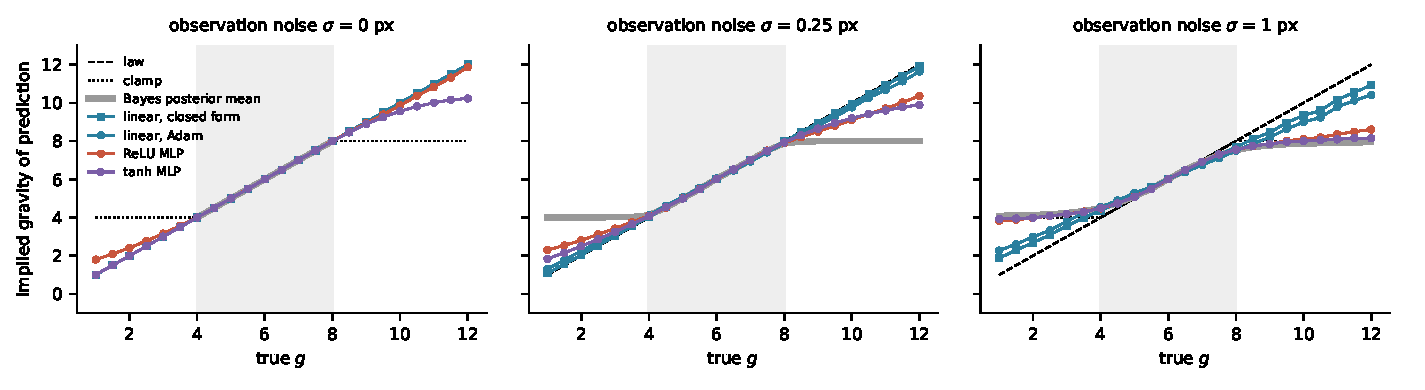
\includegraphics[width=\textwidth]{fig_toy.pdf}
\caption{Proposition~\ref{prop:clamp} in the simplest setting: 1D free fall, ten noisy context heights,
twenty future heights, squared loss, $g\sim\mathcal U[4,8]$ at training. The grey curve is the exact
posterior mean. A linear predictor (for which the law is linear in the data) extrapolates the law
when there is no noise, because then the loss does not constrain out-of-range contexts and the
least-norm solution happens to be the law; with noise its implied gravity follows the posterior
mean. ReLU and tanh MLPs trained on the same data clamp even without noise. Mean of 3 seeds.}
\label{fig:toy}
\end{figure*}

\paragraph{Consequences for experiments.} Proposition~\ref{prop:clamp} gives a reference curve
for OOD gravity. Figure~\ref{fig:toy} shows the proposition at work in a toy setting where
everything is exact; the caption is written before the toy results and may need revision.
% FINALIZE: rewrite the caption from results/v2/toy_bayes.json. The \emph{law} is $g_{\rm eff} = g^\star$, and the \emph{Bayes-optimal}
response is approximately $\mathrm{clamp}(g^\star, a, b)$, softened by noise
(Fig.~\ref{fig:locus}a shows the exact truncated-normal curve for our contexts). A model that
snaps back is therefore doing what its loss asks. A model that extrapolates does so because of an
inductive bias that the loss does not specify. Two further points matter for interpreting
interventions. First, the Bayes predictor can be built so that its belief state stores the
\emph{unclamped} sufficient statistic $\hat g_n$ and applies the clamp only when it predicts.
Clamping can therefore live in ``inference'' or in ``execution'', and the theory does not say
which. That is an empirical question, and Section~\ref{sec:locus} answers it with probes and
steering. Second, (iii) means that what happens out of range is decided by the architecture's
extrapolation behaviour. ReLU and GRU networks are known to extrapolate roughly linearly along
some directions \citep{xu2021extrapolate}, so partial extrapolation is a priori plausible.

\section{Setup}
\label{sec:setup}

\paragraph{World.} A 2D unit box, periodic in $x$, with a floor and a ceiling
(Fig.~\ref{fig:world}). It holds 1--3 objects, either balls (radius $0.06$--$0.10$) or
non-rotating square blocks (half-size $0.05$--$0.085$). Mass equals area, so mass is visible. Each
episode draws its own gravity $g\sim\mathcal{U}[4,8]$, restitution $e$ ($e{=}1$ with probability
$\tfrac12$, otherwise $\mathcal U[0.6,1)$) and floor/ceiling friction $\mu$ ($0$ with probability
$\tfrac12$, otherwise $\mathcal U[0.05,0.4]$). Object colors are random and distinct. The simulator
integrates ballistic motion exactly, resolves floor and ceiling impacts at the exact time of
impact, and uses impulses for object contacts. Horizontal momentum is therefore exactly conserved
when $\mu{=}0$, and energy is conserved to $<6\times10^{-4}$ relative error over 72 frames when
$e{=}1,\mu{=}0$ (unit tests). Episodes have 40 frames at 25\,fps, rendered at $64{\times}64$ on the
GPU. Ground-truth state, energy and momentum are stored per frame. The training set has 16k
episodes. Out-of-distribution (OOD) sets vary one factor: gravity $g\in\{1,1.5,\dots,12\}$
(\texttt{gsweep}), object count 4--5, speed 2.2--4.2, and a $12{\times}$ mass ratio.

\paragraph{Models.} All models share a recurrent core, a Dreamer-style deterministic latent
imagination loop \citep{hafner2020dreamer}. A per-frame encoder gives a 64-d latent $z_t$
(layer-normalized). A GRU consumes $z_1,\dots,z_8$ (context), producing the \emph{belief state}
$h_C$. It then runs open loop on its own predictions $\hat z_{t+1} = \mathrm{head}(h_t)$. The three
families differ only in perception and training signal:
\textbf{REC}, a CNN encoder and deconvolutional decoder trained by (foreground-weighted) pixel
reconstruction of open-loop predictions;
\textbf{JEPA}, the same CNN encoder trained to predict the latents of an EMA target encoder with
VICReg variance/covariance regularization \citep{bardes2022vicreg,grill2020byol} and no decoder;
\textbf{STATE}, an MLP encoder of ground-truth object positions (no velocities, no parameters),
i.e.\ perfect perception with the same inference problem. Training uses 32-frame windows with
8 context and 24 open-loop steps, 8k AdamW steps and batch 16. Sizes S/M/L have CNN width
16/32/64 and GRU width 128/256/512 (0.7M/2.2M/7.8M parameters for REC).

\paragraph{Reading physics out of a model.} We never trust a model's own readout of physics.
Predicted latents are decoded to frames. For JEPA we use a decoder fit \emph{post hoc} on frozen
target-encoder latents of held-out frames, so it cannot shape the representation. Object
positions are then soft color-assignment centroids, with sub-pixel error on true frames
(median $<0.3$\,px, tested). The \emph{effective gravity} $g_{\rm eff}$ of a rollout is the
median of $-2\times$ the curvature of quadratic fits to 7-frame windows in which an object is in
free flight according to its own predicted track. On true frames this recovers $g$ with slope
$1.00$ (tested).

\paragraph{Three measurements of gravity.} For each model we measure gravity three ways.
\begin{itemize}
\item \textbf{Natural response.} $g_{\rm eff}$ of open-loop rollouts from real \texttt{gsweep} contexts.
\item \textbf{Internal estimate.} A ridge probe $\hat g(h) = w^\top h + b$ fit on in-range
validation contexts, applied to $h_C$ on \texttt{gsweep}.
\item \textbf{Execution.} We \emph{write} a gravity into the belief state and measure what the
rollout does. The encoding direction $u_g$ is estimated from \emph{matched-state counterfactual
pairs}. Because conservative dynamics are time-reversible, we can construct two contexts that end
in exactly the same state but were generated under different gravities $g, g' \in [4,8]$, by
simulating the velocity-reversed state backwards. Then
$u_g = \mathbb E[(h_C(g') - h_C(g))/(g'-g)]$. Unlike a probe's decoding weights
\citep{haufe2014interpretation}, $u_g$ is the change in belief caused by gravity alone,
with the present state held fixed exactly. To steer, we set
$h_C \leftarrow h_C + \delta u_g$ with $\delta$ chosen so that $\hat g$ reads a target
$g^\star\in\{1,\dots,12\}$, roll out, and measure $g_{\rm eff}$.
\end{itemize}
For a response curve $v(g)$ we report the in-range slope $s$ (over $[4,8]$) and the normalized
out-of-range slopes $\rho_{\rm hi} = (\bar v(12)-\bar v(8))/(4s)$ and
$\rho_{\rm lo} = (\bar v(4)-\bar v(1))/(3s)$. Here $\rho{=}1$ means the law is extrapolated and
$\rho{=}0$ means the response clamps at the training boundary. Steering is valid only if it
transfers in range ($s_{\rm exe}\ge0.5$) and moves rollouts toward the simulator's counterfactual
from the same state. The latter is measured by the counterfactual error reduction
$\mathrm{CER} = 1 - \mathrm{err}(\text{steered}, \tau^\star)/\mathrm{err}(\text{unsteered},\tau^\star)$.

\paragraph{Locus rule (pre-registered).} The failure on a side (high or low) is
\emph{inference-limited} if steered rollouts extrapolate further than natural ones (CI of
$\rho_{\rm exe}-\rho_{\rm nat}$ above 0) and $\rho_{\rm exe}\ge 0.5$. It is
\emph{execution-limited} if $\rho_{\rm exe}<0.5$ with its CI below 0.5. Otherwise it is mixed.

\paragraph{Statistics.} The unit of replication is the training run. We train 3 seeds for the main
M-size models and 2 seeds for each scaling cell. CIs are hierarchical bootstrap intervals
(resample seeds, then episodes; 2000 resamples). The 10 confirmatory tests are Holm-corrected.
Hypotheses, metrics and tests were committed before any model was trained
(\texttt{PREREGISTRATION.md}); every deviation is logged there.

\section{Results}
\label{sec:results}

All numbers are generated from \texttt{results/v2/summary.json}; intervals are 95\% hierarchical
bootstrap CIs. Analyses added after pre-registration are marked exploratory. Example episodes and predictions are in
\Cref{fig:world} (Appendix~\ref{app:extra}).


\begin{figure*}[t]
\centering
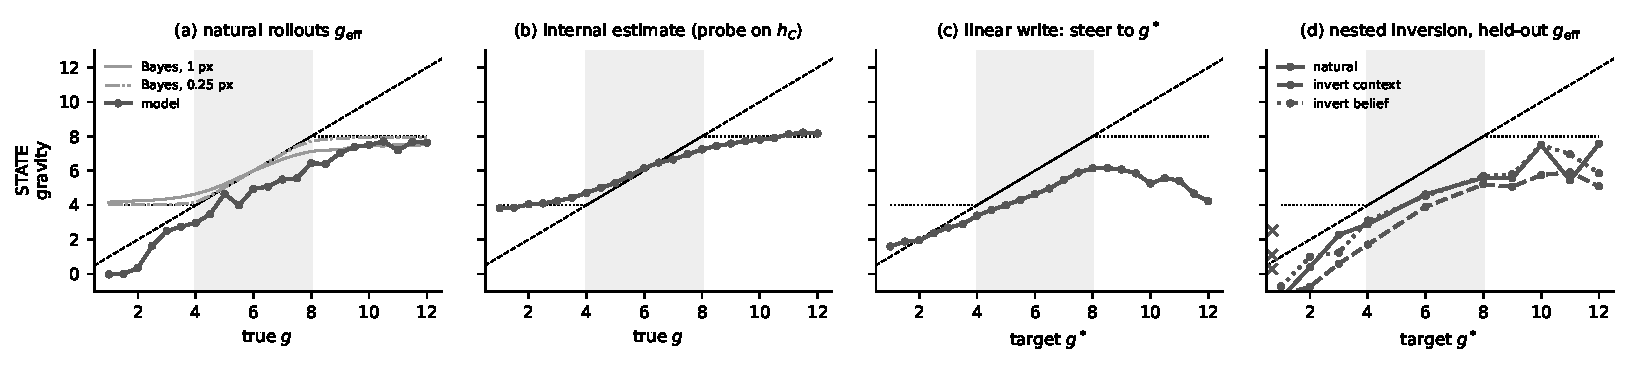
\includegraphics[width=0.72\textwidth]{fig_locus.pdf}
\caption{Where the out-of-range failure lives. Rows: families. (a) Natural predictions, with the
Bayes-optimal reference (grey). (b) The gravity a linear probe reads from the belief. (c) Linear
write: predictions after steering the belief so that the probe reads $g^\star$. (d) Nested inversion
on held-out frames: natural, inverted context latents and inverted belief; the crosses at the left
are the anti-physics control ($g=-4$). Dashed: the law; dotted: the clamp.}
\label{fig:locus}
\end{figure*}

\subsection{Competence gate and decodability (E0, E1)}
\label{sec:competence}

\Cref{tab:competence} reports the pre-registered competence gate (in-range slope of
$g_{\rm eff}$ against $g$ on validation episodes) and probe decodability. STATE \StateGate{} the
gate (slope \StateSlope), REC \RecGate{} (\RecSlope) and JEPA \JepaGate{} (\JepaSlope).
Gravity is linearly decodable from the trained belief at $R^2$ \StateRtwoG{} (STATE), \RecRtwoG{}
(REC) and \JepaRtwoG{} (JEPA), against \StateRtwoGun{}, \RecRtwoGun{} and \JepaRtwoGun{} for an
untrained dynamics network on the same inputs. H1 demanded $R^2\ge 0.5$ and is supported only for
STATE (Holm $p$: \PHOneState, \PHOneRec, \PHOneJepa). Energy at the last context frame is
decodable at $R^2$ \StateRtwoE{}, \RecRtwoE{} and \JepaRtwoE{} (Appendix~\ref{app:extra}), as
Proposition~\ref{prop:decode} predicts for any competent predictor.

\begin{table}[t]
\centering\small
\caption{Competence and decodability (M size, $10^5$ episodes, mean over seeds).}
\label{tab:competence}
\setlength{\tabcolsep}{3pt}
\begin{tabular}{lcccccc}
\toprule
Family & seeds & slope & err$_8$ (px) & $R^2_g$ & $R^2_g$ untr. & $R^2_E$\\
\midrule
STATE & \StateSeeds & \StateSlope & \StateErrEight & \StateRtwoG & \StateRtwoGun & \StateRtwoE\\
REC   & \RecSeeds   & \RecSlope   & \RecErrEight   & \RecRtwoG   & \RecRtwoGun   & \RecRtwoE\\
JEPA  & \JepaSeeds  & \JepaSlope  & \JepaErrEight  & \JepaRtwoG  & \JepaRtwoGun  & \JepaRtwoE\\
\bottomrule
\end{tabular}
\end{table}


\subsection{Natural out-of-range response (E2)}
\label{sec:natural}

\Cref{fig:locus}(a) shows the gravity that natural predictions exhibit as the true gravity sweeps
from 1 to 12, together with the Bayes-optimal reference of Proposition~\ref{prop:clamp}. The
pre-registered normalized slopes ($1$ = law, $0$ = clamp) are
$\rho_{\rm hi}=$ \StateNatHi{} for STATE, \RecNatHi{} for REC and \JepaNatHi{} for JEPA.
H2 predicted $\rho<0.5$ on both sides and is \emph{not supported} for any family (\Cref{tab:hyp}, Appendix~\ref{app:extra}).
On the high side the STATE estimate is below 0.5 but its interval crosses it, and the pixel-family
intervals are too wide to say anything. On the low side the estimates exceed one
(\StateNatLo, \RecNatLo, \JepaNatLo). This is an artifact: at low gravity the models predict floor contacts that the slow reference
never makes, and the curvature fit reads them as extra acceleration (Appendix~\ref{app:details}).

The exploratory law fraction $\lambda$ (Appendix~\ref{app:lambda}; projection of the prediction onto the law-minus-clamp
counterfactual difference; all frames, no curvature fit) gives a tighter and plainer picture
(\Cref{tab:lambda}). On the high side natural predictions sit roughly half-way between clamp and
law: \StateLambdaNatHi{} (STATE), \RecLambdaNatHi{} (REC), \JepaLambdaNatHi{} (JEPA). On the low
side they sit near the clamp: \StateLambdaNatLo{}, \RecLambdaNatLo{}, \JepaLambdaNatLo. The models
neither clamp as the noisy-Bayes reference does nor follow the law, and they extrapolate upward
better than downward.


\begin{table}[t]
\centering\small
\caption{Exploratory law fraction $\lambda$ (1 = law, 0 = clamp). ``nat'' and ``write'' use all 20
predicted frames; the last four columns use only the held-out frames 4--13 of the inversion
episodes. WIDE is the same architecture trained on $g\sim\mathcal U[1,12]$ (one seed): an
empirical ceiling.}
\label{tab:lambda}
\setlength{\tabcolsep}{3.5pt}
\begin{tabular}{llcccccc}
\toprule
 & & \multicolumn{2}{c}{all frames} & \multicolumn{4}{c}{held-out frames}\\
\cmidrule(lr){3-4}\cmidrule(lr){5-8}
side & family & nat & write & nat & inv-$z$ & inv-$h$ & WIDE\\
\midrule
high & STATE & \StateLamNatHiPt & \StateLamSteerHiPt & \StateHoldNatHi & \StateHoldInvZHi & \StateHoldInvHHi & \StateHoldWideHi\\
     & REC   & \RecLamNatHiPt & \RecLamSteerHiPt & \RecHoldNatHi & \RecHoldInvZHi & \RecHoldInvHHi & \RecHoldWideHi\\
     & JEPA  & \JepaLamNatHiPt & \JepaLamSteerHiPt & \JepaHoldNatHi & \JepaHoldInvZHi & \JepaHoldInvHHi & \JepaHoldWideHi\\
\midrule
low  & STATE & \StateLamNatLoPt & \StateLamSteerLoPt & \StateHoldNatLo & \StateHoldInvZLo & \StateHoldInvHLo & \StateHoldWideLo\\
     & REC   & \RecLamNatLoPt & \RecLamSteerLoPt & \RecHoldNatLo & \RecHoldInvZLo & \RecHoldInvHLo & \RecHoldWideLo\\
     & JEPA  & \JepaLamNatLoPt & \JepaLamSteerLoPt & \JepaHoldNatLo & \JepaHoldInvZLo & \JepaHoldInvHLo & \JepaHoldWideLo\\
\bottomrule
\end{tabular}
\end{table}

\subsection{Locating the failure (E3)}
\label{sec:locus}

\paragraph{Internal estimate.} The probe's reading of out-of-range gravity
(\Cref{fig:locus}b) has normalized slope
(\Cref{fig:locus}b) is the best-measured quantity in the study. Its normalized slope is
\StateInfHi{} (STATE), \RecInfHi{} (REC) and \JepaInfHi{} (JEPA) on the high side, and
\StateInfLo{}, \RecInfLo{}, \JepaInfLo{} on the low side. The belief tracks out-of-range gravity
but under-reads it: by about half above the range and by about a third below it. On the high side
this matches what the predictions do ($\lambda\approx 0.5$--$0.7$), so there the belief holds no
more than the output shows. On the low side the belief reads far more gravity change than the
predictions express ($\lambda\le 0.3$): information is present and unused. One caveat: a linear
probe fit in range under-reads by a similar factor on frozen V-JEPA~2 features of the same frames
(\VjRhoHi{} on the high side; Appendix~\ref{app:extra}), so part of the under-reading may be the
geometry of the code and not a clamped belief.

\paragraph{Linear write.} Steering along the matched-pair direction transfers in range with slope
$s_{\rm exe}=$ \StateExeS{} (STATE), \RecExeS{} (REC), \JepaExeS{} (JEPA), and reduces the error
to the simulator's counterfactual by CER $=$ \StateCer{}, \RecCer{}, \JepaCer{}. H3 (validity of
the write) is supported only for STATE (Holm $p$: \PHThreeState, \PHThreeRec, \PHThreeJepa), so we
interpret steering only there. For STATE, writing the true gravity raises the high-side law fraction
from \StateLamNatHiPt{} to \StateLamSteerHiPt, the level of the WIDE model trained on that range
(\StateWideLamHi). On the low side it moves only from \StateLamNatLoPt{} to \StateLamSteerLoPt{}
(WIDE: \StateWideLamLo).

\paragraph{Nested inversion.} The pre-registered inversion slopes do not resolve anything. With the
belief optimized (inv-$h$), held-out $\rho_{\rm hi}$ is \StateInvHHi{} (STATE), \RecInvHHi{} (REC)
and \JepaInvHHi{} (JEPA), and the other cells are as wide. The pre-registered decision
rule returns \StateLocusHi/\RecLocusHi/\JepaLocusHi{} above the range and
\StateLocusLo/\RecLocusLo/\JepaLocusLo{} below it (STATE/REC/JEPA). We report the labels because we committed to them and do not lean on them: across the 21
configurations of Appendix~\ref{app:extra} they change with no pattern.

In the law fraction on the same held-out frames (\Cref{tab:lambda}, right) the picture is
asymmetric. On the low side, optimizing the belief helps every family (STATE
\StateHoldNatLo{}$\to$\StateHoldInvHLo, REC \RecHoldNatLo{}$\to$\RecHoldInvHLo, JEPA
\JepaHoldNatLo{}$\to$\JepaHoldInvHLo): beliefs exist that make the frozen decoder continue a
low-gravity trajectory better than the natural belief does, and for STATE the frozen belief network
does not reach them from any context latents we could find (inv-$z$ \StateHoldInvZLo). On the high
side inversion gains little for STATE (\StateHoldNatHi{}$\to$\StateHoldInvHHi) and loses for the
pixel families. The anti-physics control reaches $\lambda=$ \StateAntiLam, \RecAntiLam{} and
\JepaAntiLam{} of the way to an upward-gravity trajectory on held-out frames. The decoder can be
bent a third of the way toward dynamics it has never seen, which bounds how much of any inversion
gain can be credited to stored physics.

\paragraph{An empirical ceiling (exploratory).} The WIDE model shows what this architecture does
when the same gravities are in range. Its in-range error equals the main model's (STATE
\StateInErrWide{} vs \StateInErr{} px; REC \RecInErrWide{} vs \RecInErr), so the wider prior costs
nothing. Out of range the main models lose \StateOodErrHi{} vs \StateOodErrWideHi{} px (STATE, high)
and \StateOodErrLo{} vs \StateOodErrWideLo{} px (low). Even WIDE reaches only $\lambda=$ \StateHoldWideHi{} on
held-out frames, so a quarter of the ``law'' is beyond this architecture at any range. Of the gap
between the natural model and WIDE, the optimized belief closes \StateGapHHi{} (high) and
\StateGapHLo{} (low) for STATE, \RecGapHLo{} (low) for REC and \JepaGapHLo{} (low) for JEPA.

\paragraph{Reading.} No single locus survives. The evidence splits the failure in two. Part is
\emph{inference}: the belief under-reads out-of-range gravity, tightly measured, in every family.
Part is \emph{execution}: even the best belief we can find closes about half of the gap to a
model trained on the range, or less. The one validated write (STATE, high side) recovers the ceiling, which suggests that this
family's high-side failure is mostly inference; inversion cannot confirm it, because a
four-frame fit barely constrains gravity. On the low side execution is the larger part.

\paragraph{Perception is not the locus.} Positions read from context latents of out-of-range
episodes exceed the in-range readout error by \RecPercExcess{} px (REC) and \JepaPercExcess{} px
(JEPA) (H5 supported).

\subsection{Scale and controls (E7)}
\label{sec:scaling}

\Cref{fig:scaling} (Appendix~\ref{app:extra}) varies the training pool from $10^3$ to $10^5$ episodes. In-range error falls by
about two pixels per decade in every family (\StateHfourErr; \RecHfourErr; \JepaHfourErr).
The slope of $\rho_{\rm hi}$ per decade is \StateHfourRho{} (STATE), \RecHfourRho{} (REC) and
\JepaHfourRho{} (JEPA). H4 required the upper bound to stay below 0.15 and is \emph{not supported}.:
we cannot claim that scale fails to buy extrapolation. The exploratory law fraction points the
other way for data. High-side $\lambda$ rises with the pool for STATE (\StateOneKLamHi,
\StateEightKLamHi{} and \StateLamNatHiPt{} at $10^3$, $8{\cdot}10^3$ and $10^5$ episodes), and the
low side leaves the clamp (\StateOneKLamLo{} to \StateLamNatLoPt). More data
bought some extrapolation here. Dynamics size did not, and a linear diagonal recurrence in place of the GRU lowered it
(STATE \StateLruLamHi; one seed each).


\subsection{Pre-registered tests}

Of seventeen confirmatory tests, four survive Holm correction (\Cref{tab:hyp}, Appendix~\ref{app:extra}): decodability and
steering validity for STATE, and the perception check for both pixel families. Secondary results (energy drift, velocity edits,
other shifts) are in Appendix~\ref{app:extra}: no family conserves energy, and we found no linear handle on
horizontal velocity.

\section{Limitations}
\label{sec:limits}

\paragraph{Scale and realism.} Our models have $10^5$--$10^7$ parameters and our world is 2D at
$64{\times}64$. We make no claim that large video generators fail in the same place. What we offer
is a method (matched-state counterfactuals, nested inversion with held-out frames, an anti-physics
calibration, a Bayes reference) and one carefully controlled answer. Applying the same dissection
to a large model requires an encoder-predictor interface whose belief state can be written into.
JEPA-style predictors have one.

\paragraph{Two-stage training.} The pixel families freeze their encoder before learning dynamics,
as World Models and V-JEPA~2-AC do. End-to-end training might place the failure differently. Our
end-to-end version-1 models never became competent at the compute we had (Appendix~\ref{app:v1}),
so we could not test this.

\paragraph{What ``execution'' means.} Inversion searches the belief space reachable by the GRU
($h=\tanh v$). A failure of inv-$h$ means that no such belief makes the frozen decoder continue an
out-of-range trajectory. It does not mean that no small change to the decoder could. The 4-frame fit
window constrains the initial curvature, so held-out success tests \emph{continuation}, not
discovery.

\paragraph{Measurement.} Effective gravity is measured only where the reference trajectory is in
free flight. At high $g$ such stretches are short and rare (about 20\% of $g{=}12$ episodes have a
qualifying stretch in the held-out window), which widens the out-of-range intervals. The
exploratory law fraction $\lambda$ uses every frame but was added after pre-registration.

\paragraph{Statistics.} Three seeds for the main models and two for scaling cells give a poor
estimate of seed-level variance. Our hierarchical bootstrap resamples seeds, but with so few seeds
its intervals are optimistic.

\paragraph{Deviations.} The study departed from its first pre-registration in substantive ways
(Appendix~\ref{app:v1}): a new world timing, visible materials, two-stage families and chunk
dynamics. All of these were committed before any version-2 evaluation. Smaller version-2 deviations
(inversion windows, sample sizes, the perception architecture of the pixel families and the
exploratory law fraction) are listed with reasons in \texttt{PREREGISTRATION\_v2.md}.

\section{Conclusion}

A world model that infers a hidden physical parameter from context and then fails outside the
training range is not necessarily broken; under squared loss, clamping to the training range is the
optimal response. Whether a model extrapolates a law is therefore a question about inductive bias,
and where it fails is a question that output behaviour and probes cannot answer. We answered it with
matched-state counterfactuals and nested inversion with held-out physics in a controlled world,
for three training signals, with pre-registered hypotheses and every deviation logged. The method
transfers to any encoder-predictor world model whose belief can be written into.


\bibliography{refs}
\bibliographystyle{icml2026}

\newpage
\appendix
\onecolumn
\section{Version 1 of this study, and why it failed}
\label{app:v1}

We pre-registered a first version (commit \texttt{6a44689}) and report its failure because the
failure modes are instructive and because hiding them would misrepresent how the final design was
reached.

\paragraph{Design.} Version 1 differed in four ways:
\begin{itemize}
\item it had 25\,fps and 8 context frames;
\item restitution and friction were hidden;
\item the training pool had 16k episodes;
\item models were trained end to end: a CNN encoder and GRU with open-loop autoregressive
prediction of 24 frames, using pixel loss (REC), EMA-target latent loss (JEPA), or ground-truth
positions (STATE); 8k steps.
\end{itemize}

\paragraph{What went wrong.}
\begin{enumerate}
\item \textbf{No competence.} All three families blurred toward the mean within about ten frames.
Linear probes recovered gravity from the belief with $R^2\approx0$. Even teacher-forced
one-step predictors on ground-truth positions did not beat a constant-velocity baseline in free
flight. Gravity's per-frame signature ($g\,\Delta t^2\approx0.6$\,px) was below the models'
precision, and the one-step loss barely rewards inferring it. Knowing the exact $g$ improves the
one-step error by about $3\times10^{-6}$, against a total loss of about $2\times10^{-3}$.
\item \textbf{Memorization.} With 16k episodes, a chunk predictor's training loss kept falling
while validation error stalled. With 200k episodes, the gap closed and probe $R^2$ for $g$ rose
from 0.2 to 0.8. In this contact-rich world, generalizing physics needs far more distinct episodes
than memorizing them does.
\item \textbf{Hidden materials dominated the loss.} With the simulator we can compute how much
prediction error each unknown causes. Not knowing $(e,\mu)$ costs 7--9\,px over 24 frames; not
knowing $g$ costs 3--5\,px. Models learned contacts long before gravity.
\item \textbf{A biased gravity estimator.} Our first $g_{\rm eff}$ estimator selected free-flight
windows from the model's own predicted track. MSE-trained models hedge on the timing of bounces.
They decelerate smoothly before an uncertain contact (a ``soft bounce''), and those windows
entered the estimate as weak or even negative gravity. Restricting the fits to frames where the
\emph{reference} trajectory is in exact free flight removes the bias.
\item \textbf{A metric bug} (a missing division by the number of frames) inflated position errors
32-fold. It was caught by inspection and pinned down by a unit test.
\end{enumerate}

Diagnosing these issues required running the full version-1 evaluation on seed-0 models, which the
version-1 pilot clause forbade. Version 2 therefore uses new splits with new seeds, and nothing from
version 1 is reported as a result. Every design change was made from train/validation diagnostics
and committed in \texttt{PREREGISTRATION\_v2.md} before any version-2 evaluation.

\section{Details}
\label{app:details}

\subsection{Effective-gravity estimator}
For an object, a \emph{run} is a maximal stretch of frames in which the reference trajectory is in
exact free flight: the second differences of its height equal $-g\,\Delta t^2$ within $2\times10^{-5}$,
with a one-frame margin on both sides of any contact. Runs of at least five frames that start within
the first eight predicted frames receive a quadratic fit in time over the predicted height; the
estimate is $-2\times$ the quadratic coefficient. Runs are combined by a weighted median, with weights
equal to the curvature precision $\sum_t q_t^2$, where $q$ is $t^2$ with the constant and linear
components projected out. On true trajectories the estimator recovers $g$ to $4\times10^{-6}$; with
i.i.d.\ Gaussian noise of 1 px on positions, its per-episode standard deviation is 0.7. At $g=12$ only
about 20\% of episodes contain a qualifying run within the held-out window (frames 4--13), because
objects reach the floor quickly; the pre-registered sample sizes account for this.

\subsection{Bayes reference}
For each \texttt{gsweep} episode, each object's longest contact-free run of context frames
(from the true trajectory) contributes Fisher information $1/s_n^2$ about $g$, where $s_n$ is the
standard deviation of the least-squares curvature estimate from $n$ noisy frames. Information is
summed across objects. The posterior under the prior $\mathcal U[4,8]$ is a truncated normal centred
on the noisy estimate; its mean is averaged over 200 draws of the noise. We report $\sigma=1$ px
(pre-registered) and $\sigma=0.25$ px.

\subsection{Matched-state counterfactual pairs}
Conservative episodes ($e=1,\mu=0$) are time-reversible. For a validation episode's state at the last
context frame, we negate velocities, simulate $C$ frames under gravity $g'$, reverse the result and
negate velocities again; this yields a context under $g'$ that ends in exactly the original state
(unit test: $<10^{-5}$). Two such contexts under $g$ and $g'$ (drawn in $[4,8]$ with $|g-g'|\ge1$)
give one pair; the encoding direction is the mean of $(h_C(g')-h_C(g))/(g'-g)$ over 800 pairs.

\subsection{Nested inversion}
inv-$h$ optimizes $v$ with $h=\tanh v$ (Adam, lr 0.05, 400 steps), starting from the natural belief,
to minimize the model's latent MSE on predicted frames 0--3 against the latents of the target
trajectory. inv-$z$ optimizes the ten standardized context latents, which are passed through the
frozen belief GRU, with the same objective. All reported metrics use frames 4--13 and runs starting
in frames 4--8. The anti-physics control uses 80 in-range contexts whose future is re-simulated from
the last context state with $g=-4$ and the episode's own $e,\mu$.

\subsection{Hyperparameters and compute}
Stage 1: 12k AdamW steps, batch 64, lr $10^{-3}$ with cosine decay, on $2.0$M-parameter (M)
encoders; JEPA uses an EMA target (0.996) and VICReg weights $(1, 0.04)$. Stage 2: 30k steps, batch
128, lr $10^{-3}$ cosine, belief width 256 and decoder width 512 for size M. Everything ran on one
laptop GPU with 4 GB of memory (RTX 3050 Ti). A stage-1 run takes about 25 minutes, a stage-2 run
about 20 minutes, and the full evaluation of one model about 10 minutes.

\subsection{Per-configuration statistics}
\begin{tabular}{lccccccc}
\toprule
Config & seeds & slope & $\rho_{\rm hi}$ nat & $\rho_{\rm hi}$ inv-$z$ & $\rho_{\rm hi}$ inv-$h$ & $\rho_{\rm lo}$ nat & locus hi / lo\\
\midrule
(no results yet) & & & & & & & \\
\bottomrule
\end{tabular}



\end{document}
